\chapter{La integral de convolución}

% corresponde al archivo sys_2023/chapter-11.tex

\section{Deducción de la fórmula}

A continuación calculamos la salida $y(t)$ para una entrada arbitraria $x(t)$ en función de la respuesta al impulso $h(t)$ del sistema lineal invariante en el tiempo.

\subsection{Una señal como límite de una sumatoria}

\begin{figure}[htbp]
	\centering
	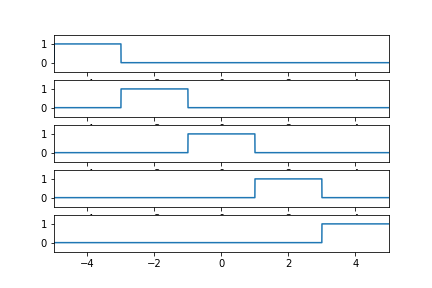
\includegraphics[width=0.7\linewidth]{graphics/pulses.png}
	\caption{Pulsos desplazados en el tiempo}
	\label{fig:pulses}
\end{figure}

\begin{figure}[htbp]
	\centering
	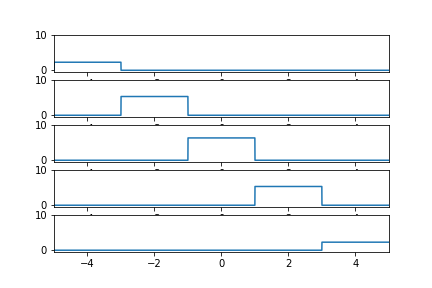
\includegraphics[width=0.7\linewidth]{graphics/modulated_pulses.png}
	\caption{Pulsos desplazados en el tiempo y modulados}
	\label{fig:modulatedpulses}
\end{figure}

\begin{figure}[htbp]
	\centering
	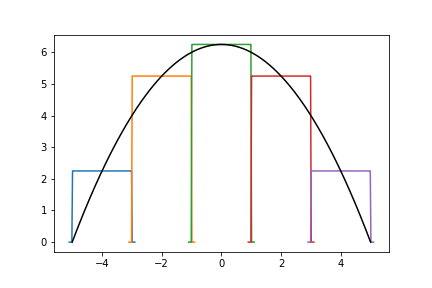
\includegraphics[width=0.7\linewidth]{graphics/coarse-approximation.png}
	\caption{Aproximación grosera}
	\label{fig:coarse-approximation}
\end{figure}

\begin{figure}[htbp]
	\centering
	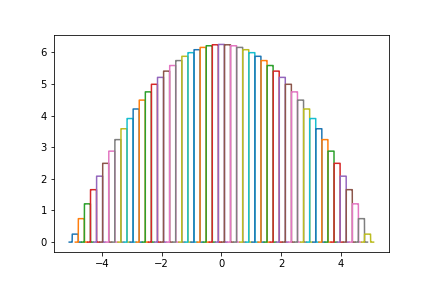
\includegraphics[width=0.7\linewidth]{graphics/fine-approximation.png}
	\caption{Aproximación fina}
	\label{fig:fine-approximation}
\end{figure}

Vamos a probar que podemos representar una señal continua como el límite de una suma de pulsos. Consideremos pulsos desplazados en el tiempo $\delta_{\Delta}\left(t - k \, \Delta \right)$ donde $\Delta$ es un incremento de tiempo variable.

Observando la figura \ref{fig:pulses}, podemos escribir las definiciones de los pulsos desplazados en el tiempo:
\begin{align}
	\vdots \nonumber \\ 
	\delta_{\Delta}(t+\Delta) &= \begin{cases}
		\frac{1}{\Delta}, & -\Delta \leq t < 0, \\ 
		0, & (t < -\Delta) \lor (0 \leq t).
	\end{cases} \\ 
	\delta_{\Delta}(t) &= \begin{cases}
		\frac{1}{\Delta}, & 0 \leq t < \Delta, \\ 
		0, & (t < 0) \lor (\Delta \leq t).
	\end{cases} \\ 
	\delta_{\Delta}(t-\Delta) &= \begin{cases}
		\frac{1}{\Delta}, & \Delta \leq t < 2\Delta, \\ 
		0, & (t < \Delta) \lor (2\Delta \leq t).
	\end{cases} \\ 
	\vdots \nonumber \\ 
	\delta_{\Delta}(t-k\Delta) &= \begin{cases}
		\frac{1}{\Delta}, & k\Delta \leq t < (k+1)\Delta, \\ 
		0, & (t < k\Delta) \lor ((k+1)\Delta \leq t).
	\end{cases}
\end{align}

Multiplicando por $x(k \, \Delta) \, \Delta$ al $k$-ésimo pulso (ver figura \ref{fig:modulatedpulses}) se obtiene:
\begin{align}
	\vdots \nonumber \\ 
	x(-\Delta) \, \delta_{\Delta}(t+\Delta) \, \Delta &= \begin{cases}
		\frac{x(-\Delta)}{\Delta} \, \Delta, & -\Delta \leq t < 0, \\ 
		0, & (t < -\Delta) \lor (0 \leq t).
	\end{cases} \\ 
	x(0) \, \delta_{\Delta}(t) \, \Delta &= \begin{cases}
		\frac{x(0)}{\Delta} \, \Delta, & 0 \leq t < \Delta, \\ 
		0, & (t < 0) \lor (\Delta \leq t).
	\end{cases} \\ 
	x(\Delta) \, \delta_{\Delta}(t-\Delta) \, \Delta &= \begin{cases}
		\frac{x(\Delta)}{\Delta} \, \Delta, & \Delta \leq t < 2\Delta, \\ 
		0, & (t < \Delta) \lor (2\Delta \leq t).
	\end{cases} \\ 
	\vdots \nonumber \\ 
	x(k\Delta) \, \delta_{\Delta}(t-k\Delta) \, \Delta &= \begin{cases}
		\frac{x(k\Delta)}{\Delta} \, \Delta, & k\Delta \leq t < (k+1)\Delta, \\ 
		0, & (t < k\Delta) \lor ((k+1)\Delta \leq t).
	\end{cases}
\end{align}

Observe que un valor dado de $t$ (por ejemplo $t_{0}$) sólo puede pertenecer a \textbf{un} intervalo $k\Delta \leq t < (k+1)\Delta$, por lo tanto, para $t_{0}$ solo uno de los productos puede ser distinto de $0$. Sumando los infinitos productos (ver figura \ref{fig:coarse-approximation}) obtenemos:
\begin{equation}
	x_{\Delta}(t) = \sum_{k=-\infty}^{\infty} x(k\Delta) \, \delta_{\Delta}(t-k\Delta) \, \Delta .
\end{equation}

Considerando la suma de los pulsos desplazados en el tiempo, podemos observar que cuando $\Delta$ tiende a cero (ver figura \ref{fig:fine-approximation}), $x_{\Delta}(t)$ tiende a $x(t)$.
\begin{equation}
	x(t) = \lim_{\Delta \to 0} x_{\Delta}(t) = \lim_{\Delta \to 0} \sum_{k=-\infty}^{\infty} x(k \, \Delta) \, \delta_{\Delta}(t-k \, \Delta) \, \Delta .
\end{equation}
Además, cuando $\Delta$ tiende a cero, la sumatoria se convierte en una integral:
\begin{equation}
	x(t) = \int_{-\infty}^{\infty} x(\tau) \, \delta(t-\tau) \, d\tau . \label{integral.convolucion}
\end{equation}

Notemos que por la propiedad del muestreo del impulso, debe cumplirse:
\begin{equation} 
	x(\tau) \, \delta(t-\tau) = x(t) \, \delta(t-\tau),
\end{equation}
y en ese caso:
\begin{equation}
	x(t) = x(t) \left( \int_{-\infty}^{\infty} \delta(t-\tau) \, d\tau \right).
\end{equation}

\subsection{La respuesta al impulso y la convolución}

Definamos $h_{k \, \Delta }(t) = h_{\Delta}\left( t-k \, \Delta \right)$ como la salida de un sistema invariante en el tiempo para el pulso $\delta_{\Delta}(t-k \, \Delta)$. 

Además, recordemos la ecuación (\ref{integral.convolucion}):
\begin{equation}
	x_{\Delta}(t) = \sum_{k=-\infty}^{\infty} x(k \, \Delta) \, \delta_{\Delta}(t-k \, \Delta) \, \Delta .
\end{equation}

La salida $y_{\Delta}(t)$ para una entrada $x_{\Delta}(t)$ puede definirse, por el principio de superposición, como:
\begin{equation}
	y_{\Delta}(t) = \sum_{k=-\infty}^{\infty} x(k\Delta) \, h_{k\Delta}(t) \, \Delta.
\end{equation}

Definamos $k\Delta = \tau$. Entonces, cuando $\Delta \to 0$, obtenemos como límite la señal $y(t)$, pero como siempre vamos a tener un $k$ suficientemente grande, $\tau$ no es necesariamente nula. Podemos escribir:
\begin{equation}
	y(t) = \lim_{\Delta \to 0} \sum_{k=-\infty}^{\infty} x(k \, \Delta) \, h_{k\Delta}(t) \, \Delta = \int_{-\infty}^{\infty} x(\tau) \, h_{\tau}(t) \, d\tau .
\end{equation}

Si el sistema es invariante en el tiempo, entonces:
\begin{equation}
	h_{\tau}(t) = h_{0}(t-\tau) ,
\end{equation}
(es decir, no importa para qué $\tau$ calculamos la respuesta, y por lo tanto elegimos $\tau=0$). Reemplazando $h_0$ simplemente por $h$, obtenemos la \textbf{integral de convolución}:
\begin{equation}
	y(t) = \int_{-\infty}^{\infty} x(\tau) \, h(t-\tau) \, d\tau .
\end{equation}

\section{Cálculo de la integral de convolución en forma gráfica}


El cálculo de la convolución tiene una interpretación gráfica.
\begin{enumerate}
	\item Consideremos la fórmula, utilizando $v$ como variable muda de integración:
	\begin{equation}
		y(t) = \int_{-\infty}^{\infty} x(v) \, h(t - v) \, dv. \label{concontgraf}
	\end{equation}
	
	\item En la Ec. (\ref{concontgraf}), el factor $h(t - v)$ es una versión de $h(v)$ invertida en el tiempo (observe el signo de la variable $v$) y desplazada por la variable independiente $t$, que es el instante para el cual deseamos calcular la salida $y(t)$.
	
	\item En base a la observación anterior, es posible enunciar la siguiente "receta" para calcular la convolución en forma gráfica:
	\begin{enumerate}
		\item Dibuje la señal $x(v)$.
		\item Invierta en el tiempo la señal $h(v)$ para obtener $h(-v)$.
		\item Repita los siguientes pasos para calcular distintos valores de $y(t)$:
		\begin{enumerate}
			\item Desplace en el tiempo la señal $h(-v)$ para obtener $h(t-v)$.
			\item Obtenga el producto $z(v,t) = x(v) \, h(t - v)$.
			\item El valor de $y(t)$ es el área bajo la curva $\int z(v,t) \, dv$.
		\end{enumerate}
	\end{enumerate}
\end{enumerate}

\section{Ejemplos}

\subsection{Convolución de una señal con un impulso desplazado}

Supongamos la entrada $x(t) = \delta(t-a)$ a un sistema lineal invariante en el tiempo con respuesta al impulso $h(t)$. En este caso la salida es:
\begin{equation}
	y(t) = \int_{-\infty}^{\infty} \delta(v - a) \, h(t - v) \, dv.
\end{equation}
Notemos que por la propiedad del impulso, el producto $\delta(v - a) \, h(t - v)$ es no nulo solo cuando $v = a$, es decir, $\delta(v - a) \, h(t - a)$. Por lo tanto:
\begin{equation}
	y(t) = \int_{-\infty}^{\infty} h(t - a) \, \delta(v - a ) \, dv = h(t - a) \left( \int_{-\infty}^{\infty} \delta(v - a ) \, dv \right).
\end{equation}
Recordemos que por definición de impulso:
\begin{equation}
	\int_{-\infty}^{\infty} \delta(v - a ) \, dv = 1.
\end{equation}
Por lo tanto:
\begin{equation}
	y(t) = h(t - a).
\end{equation}
Así comprobamos la invariancia en el tiempo de los sistemas cuya salida $y(t)$ para una entrada $x(t)$ puede calcularse con la integral de convolución.

\subsection{Dos señales infinitas}

\begin{enumerate}
	
	\item Sean dos señales definidas como:
	\begin{align}
		x(t) &= e^{2t} \, u(-t) ,  \\
		h(t) &= u(t-3).
	\end{align}
	
	\item Calculando la integral de convolución tenemos:
	\begin{equation}
		x(t) * h(t) = \int_{-\infty}^{\infty} e^{2\tau} u(-\tau) u(t-3-\tau) d\tau .
	\end{equation}
	
	\item El producto de los escalones $u(-\tau) u(t-3-\tau)$ puede analizarse así:
	\begin{enumerate}
		\item Debemos observar las transiciones de los escalones (donde cambian de $0$ a $1$ y viceversa). Estas transiciones determinan los límites de integración, porque si el integrando es nulo entonces la integral se anula.
		\item Sabemos que $u(-\tau) = 1$ para $\tau \leq 0$.
		\item Sabemos que $u(t-3-\tau) = 1$ para $\tau \leq t-3$.
		\item Por lo tanto, el integrando es no nulo cuando $\tau \leq \min(0, t-3)$.
	\end{enumerate}
	
	\item Evaluando para distintos valores de $t$:
	\begin{itemize}
		\item Para $t < 3$, el límite superior es $t-3$. 
		\begin{equation}
			x(t) * h(t) = \int_{-\infty}^{t-3} e^{2\tau} d\tau = \left[ \frac{1}{2}e^{2\tau} \right]_{-\infty}^{t-3} = \frac{1}{2}e^{2(t-3)}.
		\end{equation}
		
		\item Para $t \geq 3$, el límite superior es $0$.
		\begin{equation}
			x(t) * h(t) = \int_{-\infty}^{0} e^{2\tau} d\tau = \left[ \frac{1}{2}e^{2\tau} \right]_{-\infty}^{0} = \frac{1}{2}.
		\end{equation}
	\end{itemize}
	
\end{enumerate}

\subsection{Un par de señales limitadas en tiempo}

\begin{enumerate}
	
	\item Sean las señales:
	\begin{equation}
		x(t) = u(t) - u(t-4),
	\end{equation}
	y
	\begin{equation}
		h(t) = \cos\left( \frac{\pi t}{2}\right) \left( u(t) - u(t-4) \right).
	\end{equation}
	
	\item Planteando la integral de convolución (y aplicando la propiedad conmutativa para que el argumento complejo quede en el coseno), obtenemos:
	\begin{equation}
		x(t) * h(t) = \int_{-\infty}^{\infty} \cos\left( \frac{\pi \tau}{2}\right) \left( u(\tau) - u(\tau -4) \right) \left( u(t-\tau) - u(t-4-\tau) \right) d\tau .
	\end{equation}
	
	\item Analizando el solapamiento de ambas ventanas rectangulares de ancho 4, obtenemos los siguientes intervalos:
	\begin{align}
		t < 0, &\quad x(t) * h(t) = 0, \\
		0 \leq t < 4, &\quad x(t) * h(t) = \int_{0}^{t} \cos\left( \frac{\pi \tau}{2}\right) d\tau , \\
		4 \leq t < 8, &\quad x(t) * h(t) = \int_{t-4}^{4} \cos\left( \frac{\pi \tau}{2}\right) d\tau , \\
		t \geq 8, &\quad x(t) * h(t) = 0.
	\end{align}
	
\end{enumerate}

\subsection{Otro par de señales limitadas en tiempo}

\begin{enumerate}
	
	\item Sean dos señales definidas por:
	\begin{align}
		x(t) &= \begin{cases}
			1, & 0 \leq t < T, \\ 
			0, & (t < 0) \lor (t \geq T).
		\end{cases} \\
		h(t) &= \begin{cases}
			t, & 0 \leq t < T, \\ 
			0, & (t < 0) \lor (t \geq T).
		\end{cases}
	\end{align}
	En forma compacta usando escalones unitarios:
	\begin{align}
		x(t) &= u(t) - u(t-T) , \\
		h(t) &= t \, (u(t) - u(t-T)) .
	\end{align}
	
	\item Invirtiendo y desplazando en el tiempo una de las señales, tenemos:
	\begin{equation}
		h(t-\tau) = (t-\tau) \, (u(t-\tau) - u(t-\tau -T)) .
	\end{equation}
	
	\item Finalmente, calculamos la integral:
	\begin{equation}
		f(t) = \int_{-\infty}^{\infty} \left( u(\tau) - u(\tau-T) \right) (t-\tau) \left( u(t-\tau) - u(t-\tau-T) \right) d\tau.
	\end{equation}
	
	\item Al igual que en el ejemplo anterior, analizamos el solapamiento de la ventana $x(\tau)$ (entre $0$ y $T$) con la ventana deslizante $h(t-\tau)$ (entre $t-T$ y $t$), obteniendo la siguiente función a trozos:
	\begin{equation}
		f(t) = \begin{cases}
			0, & t < 0, \\
			\left[ t \tau - \frac{\tau^2}{2} \right]_{0}^{t} = \frac{t^2}{2}, & 0 \leq t < T, \\
			\left[ t \tau - \frac{\tau^2}{2} \right]_{t-T}^{T} = -\frac{t^2}{2} + tT, & T \leq t < 2T, \\
			0, & t \geq 2T.
		\end{cases}
	\end{equation}
	
\end{enumerate}
